\documentclass{standalone}
\usepackage{tikz}
\usetikzlibrary{patterns, positioning}
\usepackage[sfdefault]{ClearSans} %% option 'sfdefault' activates Clear Sans as the default text font
\usepackage[T1]{fontenc}

\begin{document}
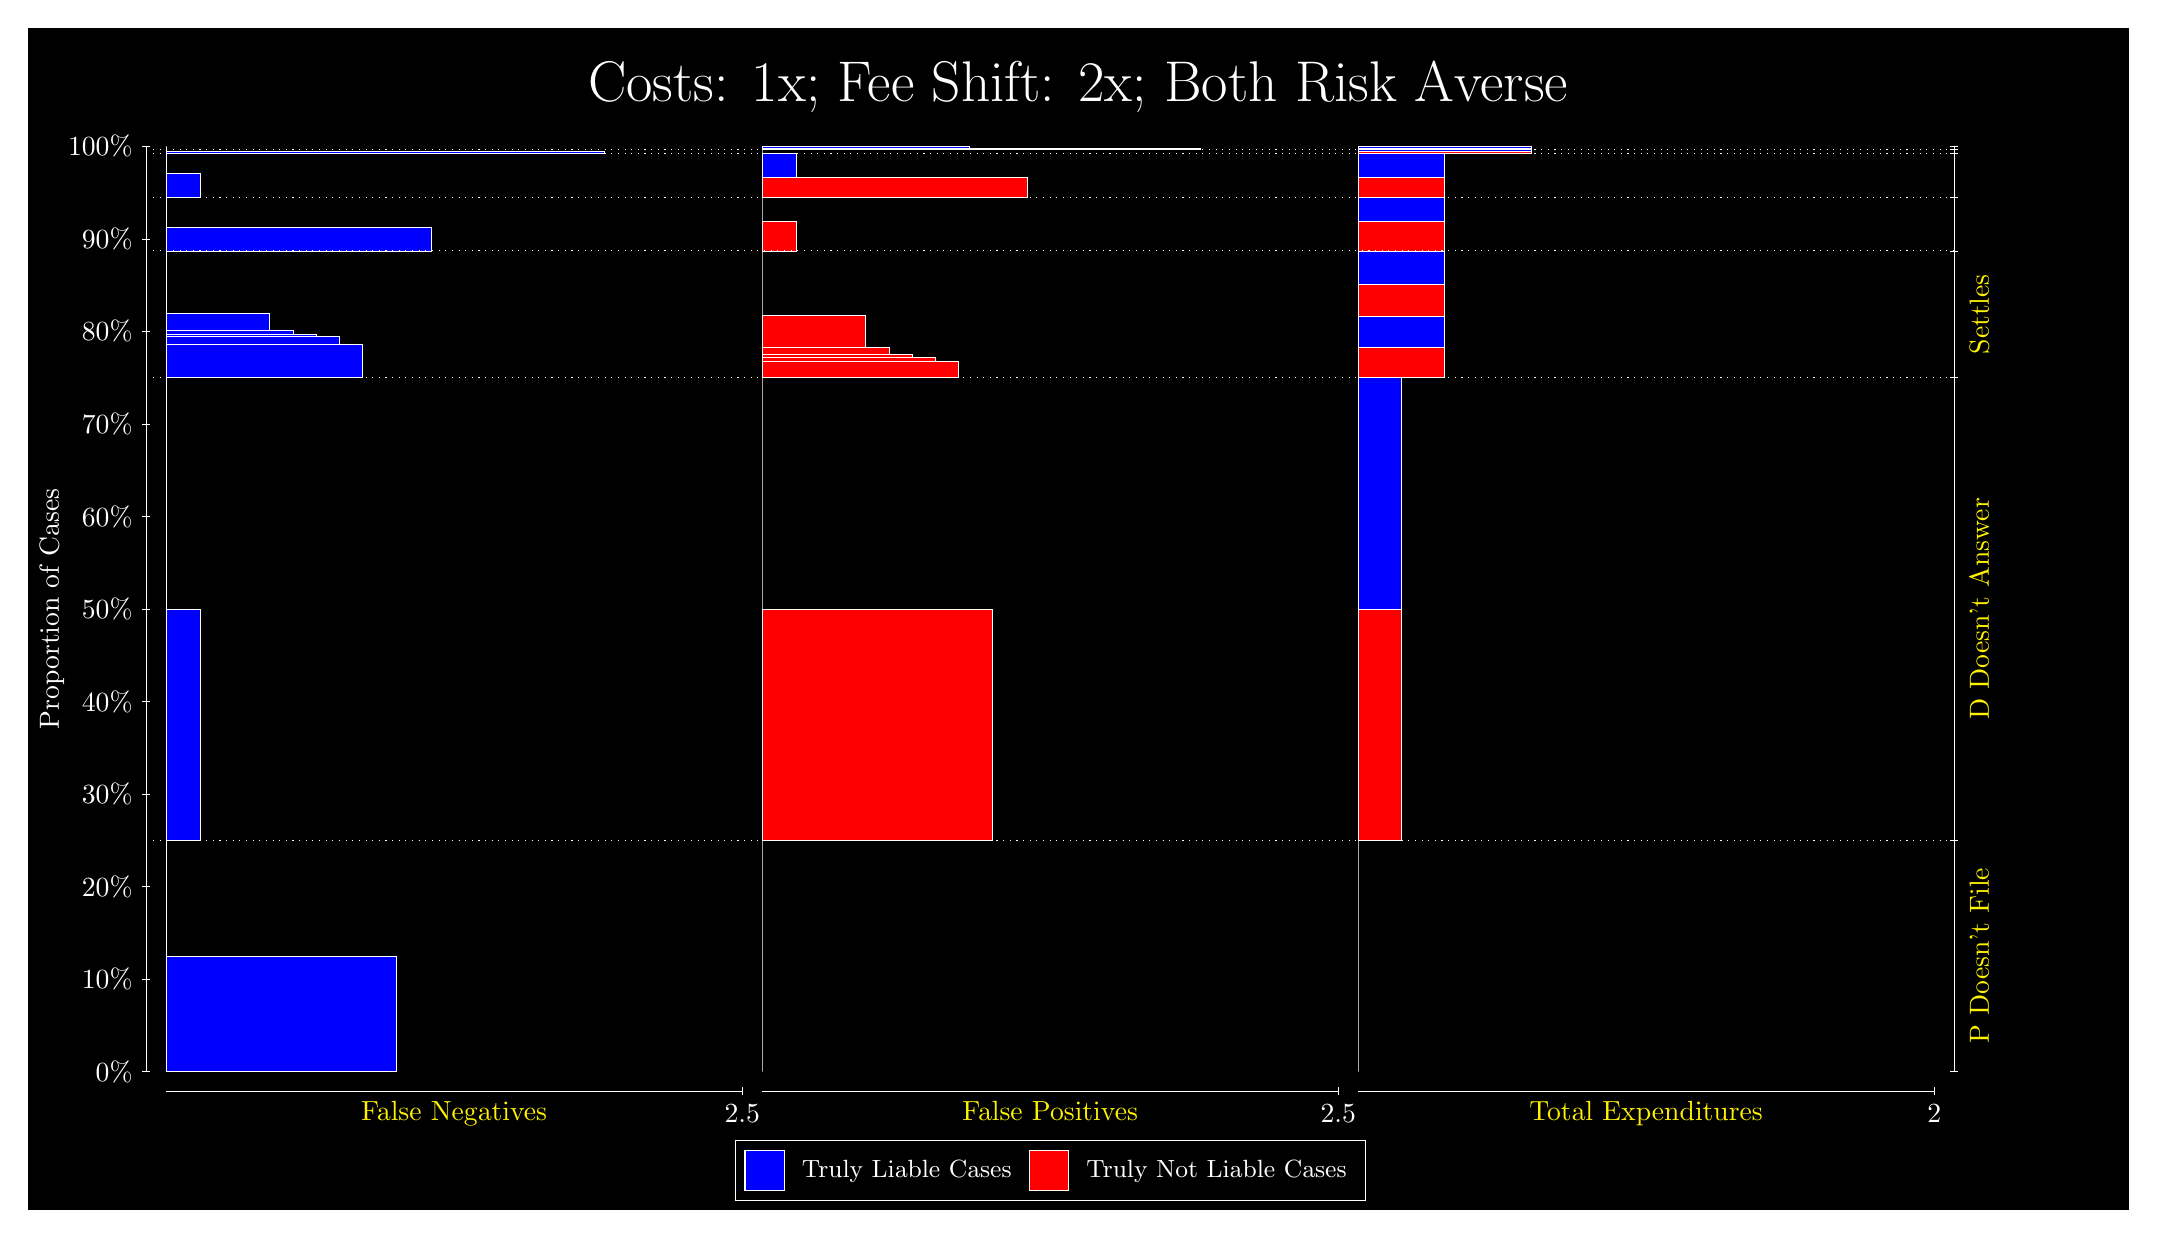
\begin{tikzpicture}
\draw[fill=black] (0,0) rectangle (26.667,15);
\draw[text=white] (0,13.5) rectangle (26.667,15) node[midway] {\huge Costs: 1x; Fee Shift: 2x; Both Risk Averse};
\draw[white, very thin] (1.5,1.75) -- (1.5,13.5);
\node[rotate=90, text=white, anchor=center] at (0.3, 7.625) {Proportion of Cases};
\draw[white, very thin] (1.45,1.75) -- (1.55,1.75);
\node[text=white, anchor=east] at (1.45, 1.75) {0\%};
\draw[white, very thin] (1.45,2.925) -- (1.55,2.925);
\node[text=white, anchor=east] at (1.45, 2.925) {10\%};
\draw[white, very thin] (1.45,4.1) -- (1.55,4.1);
\node[text=white, anchor=east] at (1.45, 4.1) {20\%};
\draw[white, very thin] (1.45,5.275) -- (1.55,5.275);
\node[text=white, anchor=east] at (1.45, 5.275) {30\%};
\draw[white, very thin] (1.45,6.45) -- (1.55,6.45);
\node[text=white, anchor=east] at (1.45, 6.45) {40\%};
\draw[white, very thin] (1.45,7.625) -- (1.55,7.625);
\node[text=white, anchor=east] at (1.45, 7.625) {50\%};
\draw[white, very thin] (1.45,8.8) -- (1.55,8.8);
\node[text=white, anchor=east] at (1.45, 8.8) {60\%};
\draw[white, very thin] (1.45,9.975) -- (1.55,9.975);
\node[text=white, anchor=east] at (1.45, 9.975) {70\%};
\draw[white, very thin] (1.45,11.15) -- (1.55,11.15);
\node[text=white, anchor=east] at (1.45, 11.15) {80\%};
\draw[white, very thin] (1.45,12.325) -- (1.55,12.325);
\node[text=white, anchor=east] at (1.45, 12.325) {90\%};
\draw[white, very thin] (1.45,13.5) -- (1.55,13.5);
\node[text=white, anchor=east] at (1.45, 13.5) {100\%};

\draw[white, very thin] (24.457,1.75) -- (24.457,13.5);
\draw[white, very thin] (24.407,1.75) -- (24.507,1.75);
\node[anchor=west] at (24.407, 1.75) {};
\draw[white, very thin] (24.407,4.6875) -- (24.507,4.6875);
\node[anchor=west] at (24.407, 4.6875) {};
\draw[white, very thin] (24.407,10.562) -- (24.507,10.562);
\node[anchor=west] at (24.407, 10.562) {};
\draw[white, very thin] (24.407,12.172) -- (24.507,12.172);
\node[anchor=west] at (24.407, 12.172) {};
\draw[white, very thin] (24.407,12.852) -- (24.507,12.852);
\node[anchor=west] at (24.407, 12.852) {};
\draw[white, very thin] (24.407,13.414) -- (24.507,13.414);
\node[anchor=west] at (24.407, 13.414) {};
\draw[white, very thin] (24.407,13.457) -- (24.507,13.457);
\node[anchor=west] at (24.407, 13.457) {};
\draw[white, very thin] (24.407,13.5) -- (24.507,13.5);
\node[anchor=west] at (24.407, 13.5) {};

\draw[white, very thin, fill=blue] (1.75,1.75) rectangle (4.6775,3.2187);
\draw[white, very thin, fill=red] (1.75,3.2187) rectangle (1.75,4.6875);
\draw[white, very thin, fill=blue] (1.75,4.6875) rectangle (2.1891,7.625);
\draw[white, very thin, fill=red] (1.75,7.625) rectangle (1.75,10.563);
\draw[white, very thin, fill=blue] (1.75,10.563) rectangle (4.2384,10.988);
\draw[white, very thin, fill=blue] (1.75,10.988) rectangle (3.9457,11.084);
\draw[white, very thin, fill=blue] (1.75,11.084) rectangle (3.6529,11.119);
\draw[white, very thin, fill=blue] (1.75,11.119) rectangle (3.3602,11.163);
\draw[white, very thin, fill=blue] (1.75,11.163) rectangle (3.0674,11.377);
\draw[white, very thin, fill=red] (1.75,11.377) rectangle (1.75,12.172);
\draw[white, very thin, fill=blue] (1.75,12.172) rectangle (5.1167,12.473);
\draw[white, very thin, fill=red] (1.75,12.473) rectangle (1.75,12.852);
\draw[white, very thin, fill=blue] (1.75,12.852) rectangle (2.1891,13.161);
\draw[white, very thin, fill=red] (1.75,13.161) rectangle (1.75,13.414);
\draw[white, very thin, fill=blue] (1.75,13.414) rectangle (7.3123,13.434);
\draw[white, very thin, fill=red] (1.75,13.434) rectangle (1.75,13.457);
\draw[white, very thin, fill=red] (1.75,13.457) rectangle (1.75,13.477);
\draw[white, very thin, fill=blue] (1.75,13.477) rectangle (1.75,13.5);
\draw[white, very thin, fill=red] (9.3189,1.75) rectangle (9.3189,3.2188);
\draw[white, very thin, fill=blue] (9.3189,3.2188) rectangle (9.3189,4.6875);
\draw[white, very thin, fill=red] (9.3189,4.6875) rectangle (12.246,7.625);
\draw[white, very thin, fill=blue] (9.3189,7.625) rectangle (9.3189,10.563);
\draw[white, very thin, fill=red] (9.3189,10.563) rectangle (11.807,10.765);
\draw[white, very thin, fill=red] (9.3189,10.765) rectangle (11.515,10.816);
\draw[white, very thin, fill=red] (9.3189,10.816) rectangle (11.222,10.857);
\draw[white, very thin, fill=red] (9.3189,10.857) rectangle (10.929,10.949);
\draw[white, very thin, fill=red] (9.3189,10.949) rectangle (10.636,11.357);
\draw[white, very thin, fill=blue] (9.3189,11.357) rectangle (9.3189,12.172);
\draw[white, very thin, fill=red] (9.3189,12.172) rectangle (9.758,12.551);
\draw[white, very thin, fill=blue] (9.3189,12.551) rectangle (9.3189,12.852);
\draw[white, very thin, fill=red] (9.3189,12.852) rectangle (12.686,13.105);
\draw[white, very thin, fill=blue] (9.3189,13.105) rectangle (9.758,13.414);
\draw[white, very thin, fill=red] (9.3189,13.414) rectangle (9.3189,13.437);
\draw[white, very thin, fill=blue] (9.3189,13.437) rectangle (9.3189,13.457);
\draw[white, very thin, fill=red] (9.3189,13.457) rectangle (14.881,13.477);
\draw[white, very thin, fill=blue] (9.3189,13.477) rectangle (11.954,13.5);
\draw[white, very thin, fill=red] (16.888,1.75) rectangle (16.888,3.2188);
\draw[white, very thin, fill=blue] (16.888,3.2188) rectangle (16.888,4.6875);
\draw[white, very thin, fill=red] (16.888,4.6875) rectangle (17.437,7.625);
\draw[white, very thin, fill=blue] (16.888,7.625) rectangle (17.437,10.563);
\draw[white, very thin, fill=red] (16.888,10.563) rectangle (17.986,10.949);
\draw[white, very thin, fill=blue] (16.888,10.949) rectangle (17.986,11.338);
\draw[white, very thin, fill=red] (16.888,11.338) rectangle (17.986,11.746);
\draw[white, very thin, fill=blue] (16.888,11.746) rectangle (17.986,12.172);
\draw[white, very thin, fill=red] (16.888,12.172) rectangle (17.986,12.551);
\draw[white, very thin, fill=blue] (16.888,12.551) rectangle (17.986,12.852);
\draw[white, very thin, fill=red] (16.888,12.852) rectangle (17.986,13.105);
\draw[white, very thin, fill=blue] (16.888,13.105) rectangle (17.986,13.414);
\draw[white, very thin, fill=red] (16.888,13.414) rectangle (19.083,13.437);
\draw[white, very thin, fill=blue] (16.888,13.437) rectangle (19.083,13.457);
\draw[white, very thin, fill=red] (16.888,13.457) rectangle (19.083,13.477);
\draw[white, very thin, fill=blue] (16.888,13.477) rectangle (19.083,13.5);
\draw[white, dotted] (1.5,4.6875) -- (24.457,4.6875);
\draw[white, dotted] (1.5,10.563) -- (24.457,10.563);
\draw[white, dotted] (1.5,12.172) -- (24.457,12.172);
\draw[white, dotted] (1.5,12.852) -- (24.457,12.852);
\draw[white, dotted] (1.5,13.414) -- (24.457,13.414);
\draw[white, dotted] (1.5,13.457) -- (24.457,13.457);
\draw[white, very thin] (1.75,1.5) -- (9.0689,1.5);
\node[text=yellow, anchor=north] at (5.4094, 1.5) {False Negatives};
\draw[white, very thin] (9.0689,1.45) -- (9.0689,1.55);
\node[text=white, anchor=north] at (9.0689, 1.45) {2.5};

\draw[white, very thin] (9.3189,1.5) -- (16.638,1.5);
\node[text=yellow, anchor=north] at (12.978, 1.5) {False Positives};
\draw[white, very thin] (16.638,1.45) -- (16.638,1.55);
\node[text=white, anchor=north] at (16.638, 1.45) {2.5};

\draw[white, very thin] (16.888,1.5) -- (24.207,1.5);
\node[text=yellow, anchor=north] at (20.547, 1.5) {Total Expenditures};
\draw[white, very thin] (24.207,1.45) -- (24.207,1.55);
\node[text=white, anchor=north] at (24.207, 1.45) {2};

\node[text=yellow, centered, rotate=90] at (24.777, 3.2188) {P Doesn't File};
\node[text=yellow, centered, rotate=90] at (24.777, 7.625) {D Doesn't Answer};
\node[text=yellow, centered, rotate=90] at (24.777, 11.367) {Settles};





\draw (12.978300999999998,1.5) node[draw=none] (baseCoordinate) {};
\begin{scope}[align=center]
        \matrix[scale=0.5, draw=white, below=0.5cm of baseCoordinate, nodes={draw}, column sep=0.1cm]{
            \node[rectangle, draw, minimum width=0.5cm, minimum height=0.5cm, fill=blue] {}; &
            \node[draw=none, font=\small, text=white] (B) {Truly Liable Cases}; &
            \node[rectangle, draw, minimum width=0.5cm, minimum height=0.5cm, fill=red] {}; &
            \node[draw=none, font=\small, text=white] (B) {Truly Not Liable Cases}; \\
            };
\end{scope}

\end{tikzpicture}
\end{document}